\documentclass{article}
    \usepackage{amssymb}
    \usepackage{color}
    \usepackage{listings}
    \usepackage{graphicx}
    \usepackage{subcaption}
    \usepackage{geometry}
    \usepackage{float}
    \geometry{
    a4paper,
    total={170mm,257mm},
    left=20mm,
    top=20mm,
    }

    \setlength{\parindent}{0em}
    \setlength{\parskip}{1em} % length of the spacing
    
    \lstset{ % General setup for the package
        language=Python,
        basicstyle=\small\sffamily,
        numbers=left,
        numberstyle=\tiny,
        frame=tb,
        tabsize=4,
        columns=fixed,
        showstringspaces=false,
        showtabs=false,
        keepspaces,
        commentstyle=\color{red},
        keywordstyle=\color{blue},
        emphstyle=\ttb\color{deepred},    
        stringstyle=\color{deepgreen}
    }
    
    \begin{document}
        \begin{figure}
            \centering
            
\includegraphics[width=0.5\linewidth]{./img/vub.png}
        \end{figure}
        \title{Modeling Languages Project Report}
        \author{Juan Jose Soriano Escobar }
        \maketitle
        \newpage

        \tableofcontents
        \newpage
    
        \begin{appendix}
            \listoffigures
          \end{appendix}
          \newpage
    
    
            \section{Introduction}

            Modeling is an important part of any System or product development that helps to understand the model system an holistic point of view and to ensure that all the functionalities and
            stakeholders requirements are cover. One of the most popular modeling tools nowadays in the software and product development environment is UML.

            UML is a communication standard for the world of software development.  It consists of different types of diagrams that will, together, help you describe the boundary of the system, the structure 
            of the system, and the behavior of the system.

            In this report, a Hospital appointment and billing system management are described and modeled in UML as result of the concepts and diagrams learn in the course of Modeling Languages.

            The description of the model in this report will be split by diagram types, covering use case, sequence, activity, state and class diagram.
             
            \newpage         
            \section{Use Case Diagram}

            A use case captures a contract between the stakeholders of a system about its behavior describes the
            system’s behavior under various conditions as it responds to a request from the “primary actor”
            (Delligatti, Steiner, & Soley, 2013). % TODO: cite

            The case diagram is also good to ensure that every member in the development team understand the main activities and behavior of the system,
            recognizing the actors and the global interactions between them

            The use case diagram is divided in three main behaviors, the appointment management, clinical history management and payments.

            \subsection{Appointment Use Case}

            In the figure \ref{fig:Appointment} the use case diagram for the appointment system is Illustrated. It contains four Actors, three Human actors such as the Patient, the Receptionist and the Doctor. 
            The remaining actor is the Hospital System which is consider as a Software from the hospital that is used to manage all the logistics, billing and service operations by different users.

            \begin{figure}[H]
                \centering 
                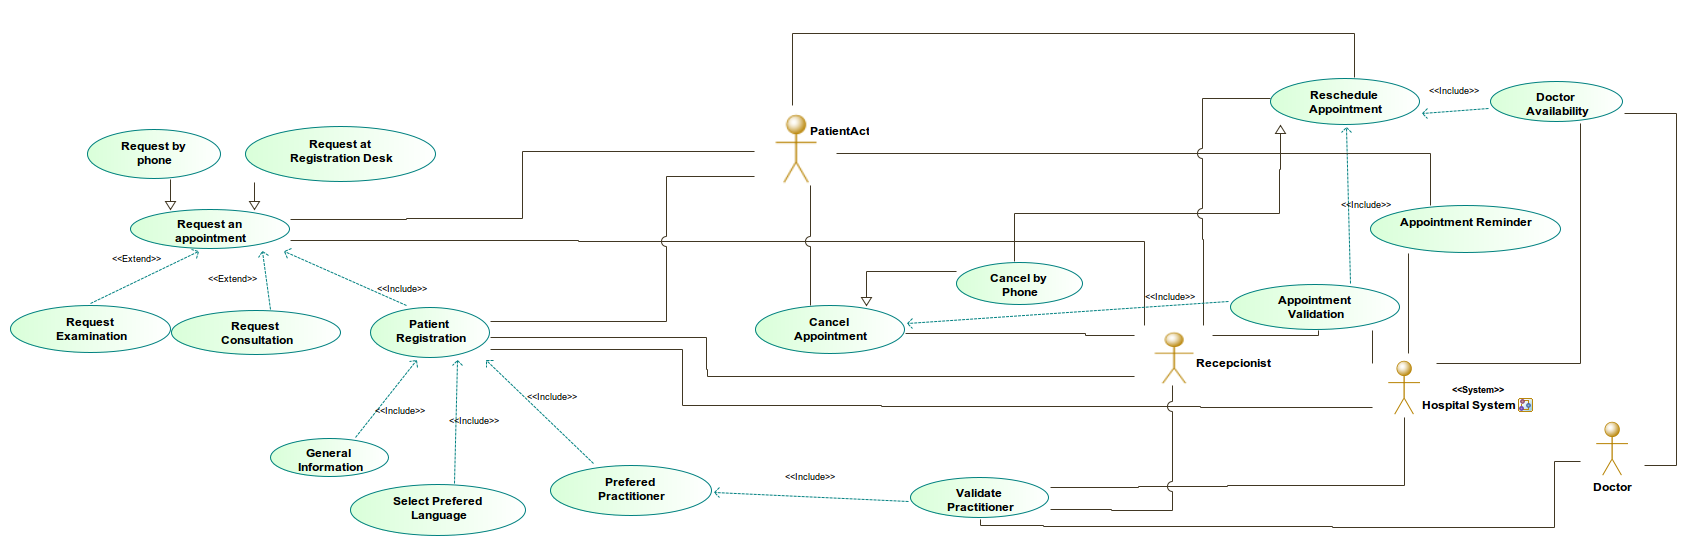
\includegraphics[width=1\linewidth]{./img/appointments.png}
                \setcaptioncitation{Created with Modelio 3.7.}
                \caption{Appoint Use Case Diagram}
                \label{fig:Appointment}
            \end{figure}


            This diagram presents how the patient communicates with the receptionist by phone or at the Hospital desk, to Schedule, cancel or modify an appointment. To do so, the Receptionist has to use the
            system, registering the patient and validating if the doctor is available for the required appointment.

            \subsection{Examination Use Case}

            Once the patient has an appointment scheduled, the next step is to understand the appointment behavior. As actors, there are the same four included in the previous Use Case Diagram plus the appointment considered as a 
            secondary one.

            The day of the appointment, the Patient will go to the Hospital desk by the time of the appointment as is expected. The receptionist will activate the appointment in the system, to let know to the Doctor and to the billing 
            staff that the patient has come to the appointment as planned.

            Once in the execution of the appointment with the Doctor, depending on the type of the appointment (Examination or consultation), the Doctor can rad and Update the Patient Clinical History by using the Hospital System. During the reportm
            the Doctor is allowed to add files, treatment description and some text explaining the patient condition.

            Other interaction between the Doctor and the system such as creating reports and email notifications will be explained later in the Sequence diagram.
            \begin{figure}[H]
                \centering 
                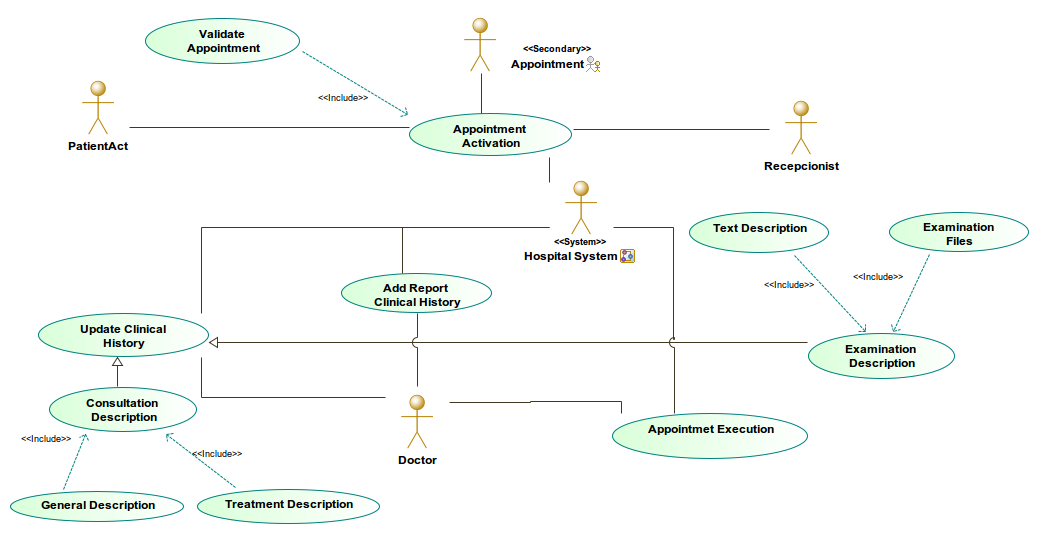
\includegraphics[width=1\linewidth]{./img/cHistories.png}
                \setcaptioncitation{Created with Modelio 3.7.}
                \caption{Examination Use Case.}
                \label{fig:examination}
            \end{figure}
            
            \subsection{Payments Use Case}

            In the payments Use Case, the appointment becomes a secondary actor by itself because the appointment is the connecting factor (somehow the product consume by the patient) between the Patient and the
            Hospital. In the diagram included in the Figure  \ref{fig:payment}, the Economy staff Actor from the hospital is introduced to review the payment status of the appointments and create penalty fees whenever is needed.
            The Economy staff uses the Hospital system to access to the appointments an patient payments.

            \begin{figure}[H]
                \centering 
                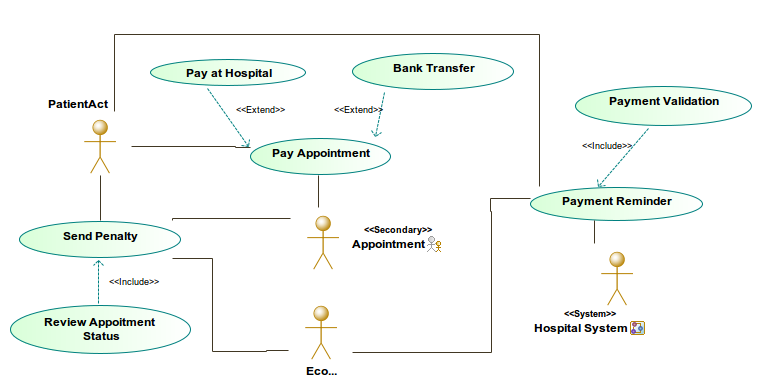
\includegraphics[width=1\linewidth]{./img/payments.png}
                \setcaptioncitation{Created with Modelio 3.7.}
                \caption{Payment Use Case Diagram}
                \label{fig:payment}
            \end{figure}

            The Patient have the option of paying at the hospital or by a bank transfer.
            
            \section{Class Diagram} %reformulate
            Class diagram describes the attributes and operations of a class and also the constraints 
            imposed on the system. The class diagrams are widely used in the modeling of objectoriented 
            systems because they are dthe only UML diagrams, which can be mapped directly with object-oriented languages.
            
            The class diagram esplain in detail the entities with it respective attributes and operations avaliable. It also describes the relation, multiplicity and
            assosiation between the the different elemets. The class diagra is one of the main elements when the system is design and the one that keep updating during the 
            design of the other diagrams.

            In the figure \ref{} the class diagram for the hospital application is presented. All the Actors in the use case diagram became entities and some sub-classes are derive from a main class.
            A good example is the Staff class that includes all thhe personal working at the Hospital in different departments. At the first level is divided in Recepcionist, Doctor Entity and Economic entity, and at the same time,
            the Doctor ebtity is generalize into Specialist, Resident and Assistance. The practitioner is considered as any of the Doctor enetities that is assign to a patient.

            Additionaly, the staff is associated to a Department and every Department contain waiting rooms that are addressed by a number, building and Section.

            As it was mentioned before, the hospital system is considered as a local software that manages the appointments and the clinic histories of the patients. In oder to access to the sytem, every member of the staff have an account with
            it respective user name and password. Iside the system the user interacts with a Graphical User Interface that displays the appointments, allow the receptionis to validate and schedule the appointments and the doctors to read and write the
            medical history of the patient. 

            The system also generates and schedule notifications. I like to imaging the system as a server runinig all the logic of the application, connected to a Databese where all the Clinical Stories, Users and bills are saved.
            The GUI is part of the front-end (and middleware) of the application and the system is the back-end, using a \textbf{token} to authenticate and stablish the connection with the database.
            
            It is easy to identify the system controller (application) as the entity with the biggest amount of operations. This is due to its "gateway" nature to allow the  interaction between the other entities and actors in the system.
            Some of the main funtions are:

            Login(String username, String password):String = It allows the user to authenticate to the system and access to the Patient, appointment and billing information. This method returns an String with the new connection view for the user. It is declare as an
            String but it could also be a XML or HTML file for a web application. The login connects to the system and use the fucntion \textit{validateFunction}.

            validateFunction(String username, String password, String token):String = This function receives the username and the password from the GUI and adds the unique token to acces and validate the user in the database. This method will return a string with the view and the
            user cookie. The cookie is assigned by the database with the function \textit{createCookie}.

            createCookie(String token, String username, String password): string =  the database system receives tghe server token toghether with the username and password and if the data is correct, it will return a acces cookie that is saved and assigned to the user in the database.
            From this point in advance I assume and is that the cookie is included by the browser or GUI in every operation while the user remains connected and authenticathed in the system.

            loginFail():String =  is an operation that is triggered when the user credentials don match with the ones created in the system.
            
            \begin{figure}[H]
                \centering 
                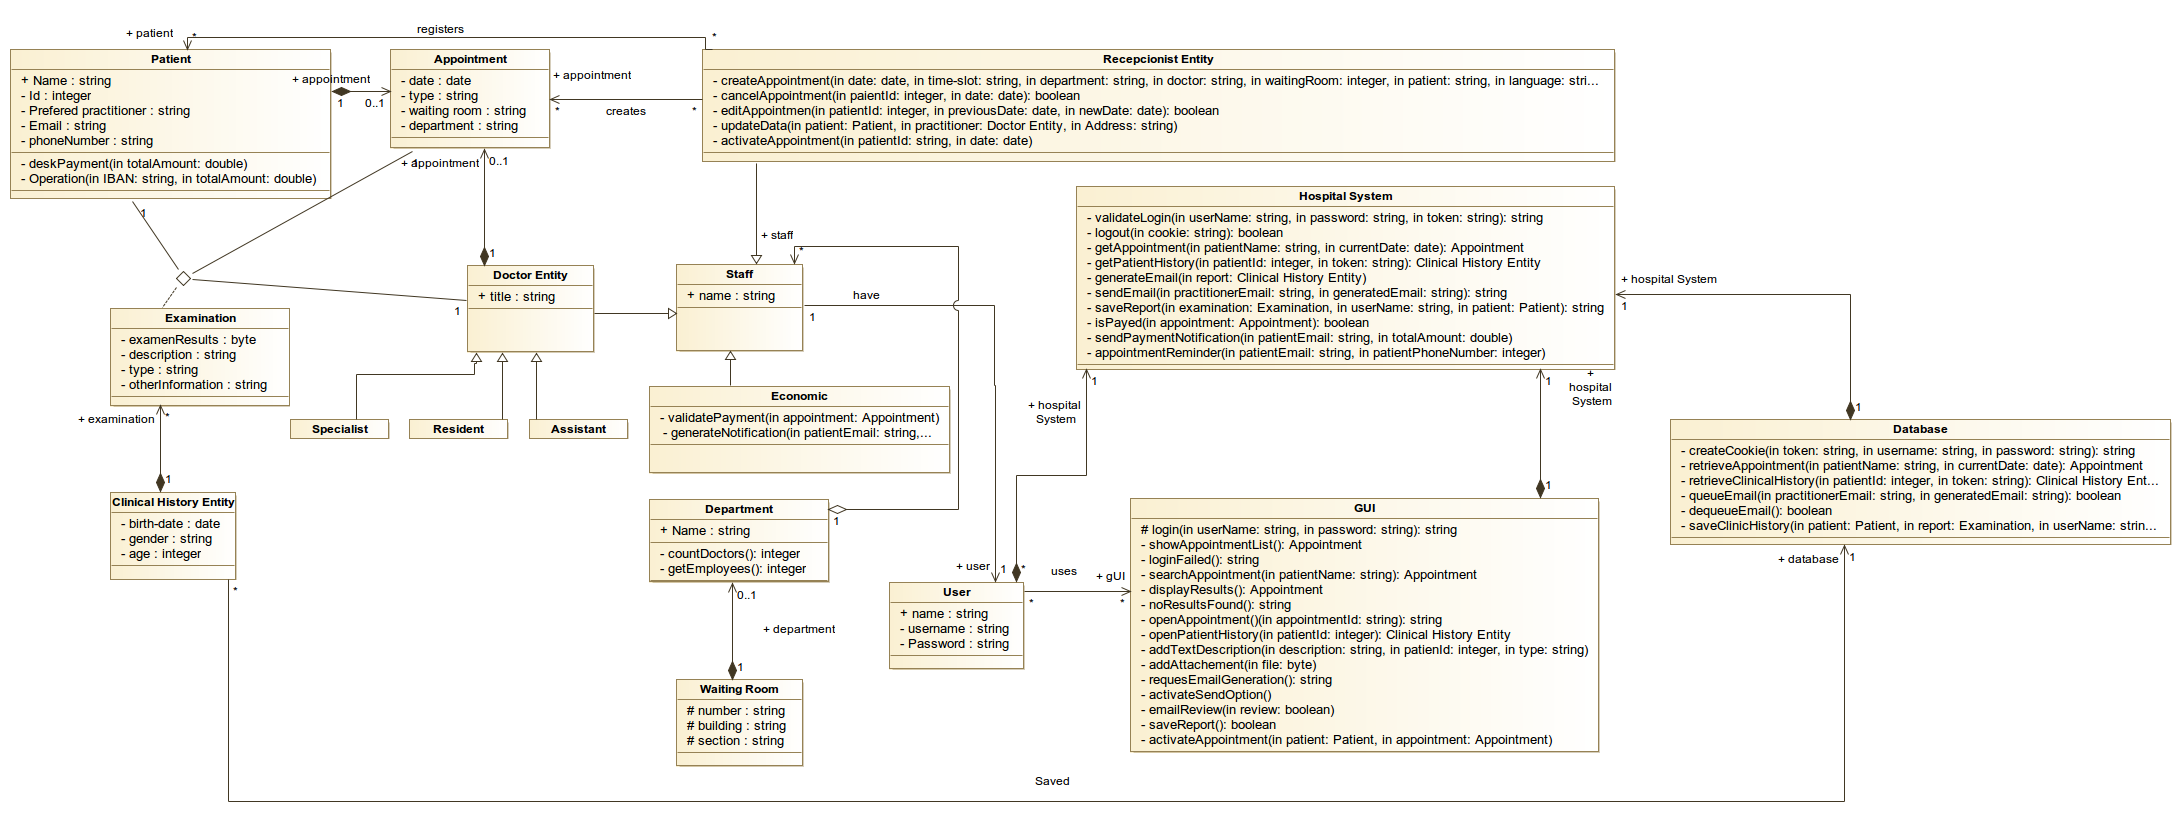
\includegraphics[width=1\linewidth]{./img/class.png}
                \setcaptioncitation{Created with Modelio 3.7.}
                \caption{Class Diagram.}
                \label{fig:class}
            \end{figure}
            \section{Sequence Diagram}
            Next to the activity diagram is the State Machine Diagram, which is also a behavior
            diagram focus on how a structure within a system changes in response to event
            occurrences over time. It refers to the behavior that begins executing the moment a block
            is instantiated and generally finishes executing when that instance is destroyed
            \begin{figure}[H]
                \centering 
                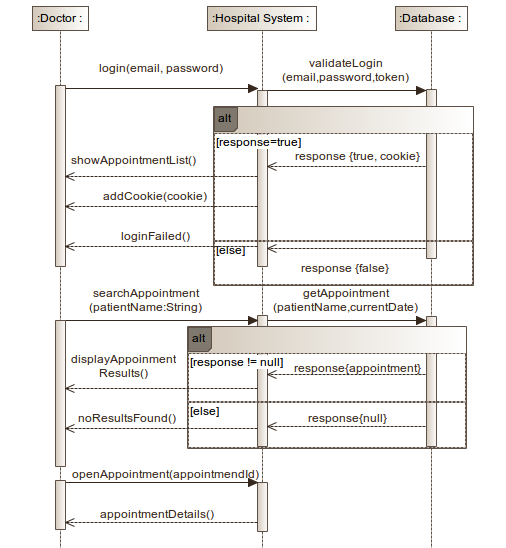
\includegraphics[width=1\linewidth]{./img/seq1.png}
                \setcaptioncitation{self-made}
                \caption{Distributed Computing Implementation.}
                \label{fig:architecture}
            \end{figure}
            \begin{figure}[H]
                \centering 
                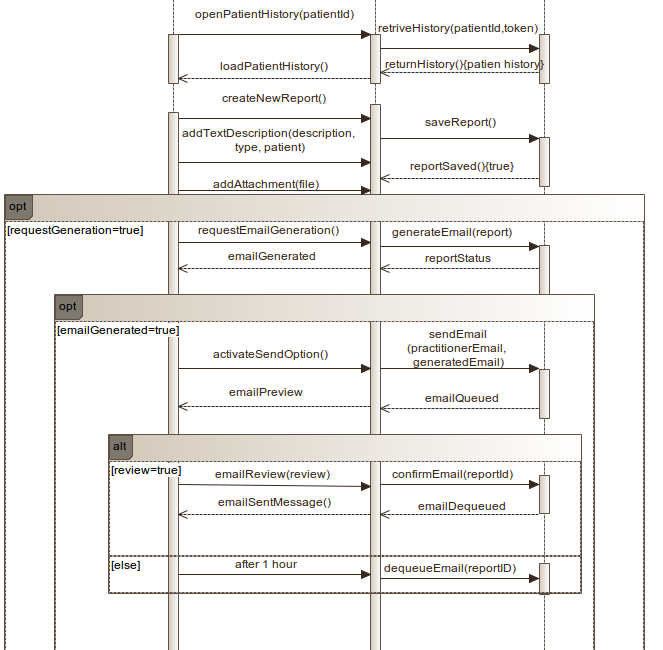
\includegraphics[width=1\linewidth]{./img/seq2.png}
                \setcaptioncitation{self-made}
                \caption{Distributed Computing Implementation.}
                \label{fig:architecture}
            \end{figure}
            \begin{figure}[H]
                \centering 
                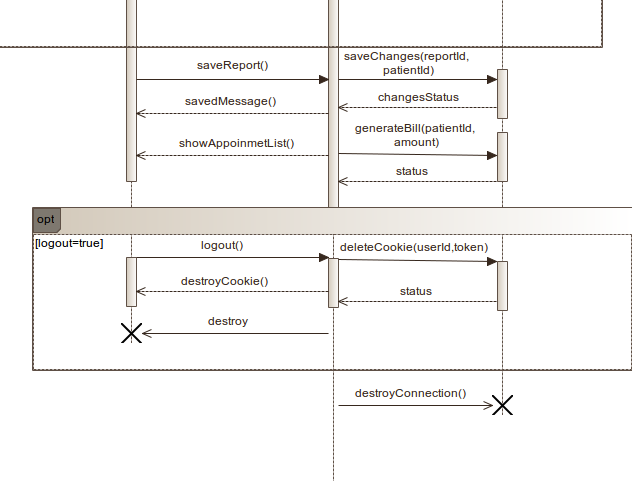
\includegraphics[width=1\linewidth]{./img/seq3.png}
                \setcaptioncitation{self-made}
                \caption{Distributed Computing Implementation.}
                \label{fig:architecture}
            \end{figure}
            \section{Activity Case Diagram}
            The activity diagrams are dynamic views of the system that expresses sequence of
            behaviors and event occurrence over time (Delligatti, Steiner, & Soley, 2013). Together
            with the state machine diagram, the system behavior is expressed.
            \begin{figure}[H]
                \centering 
                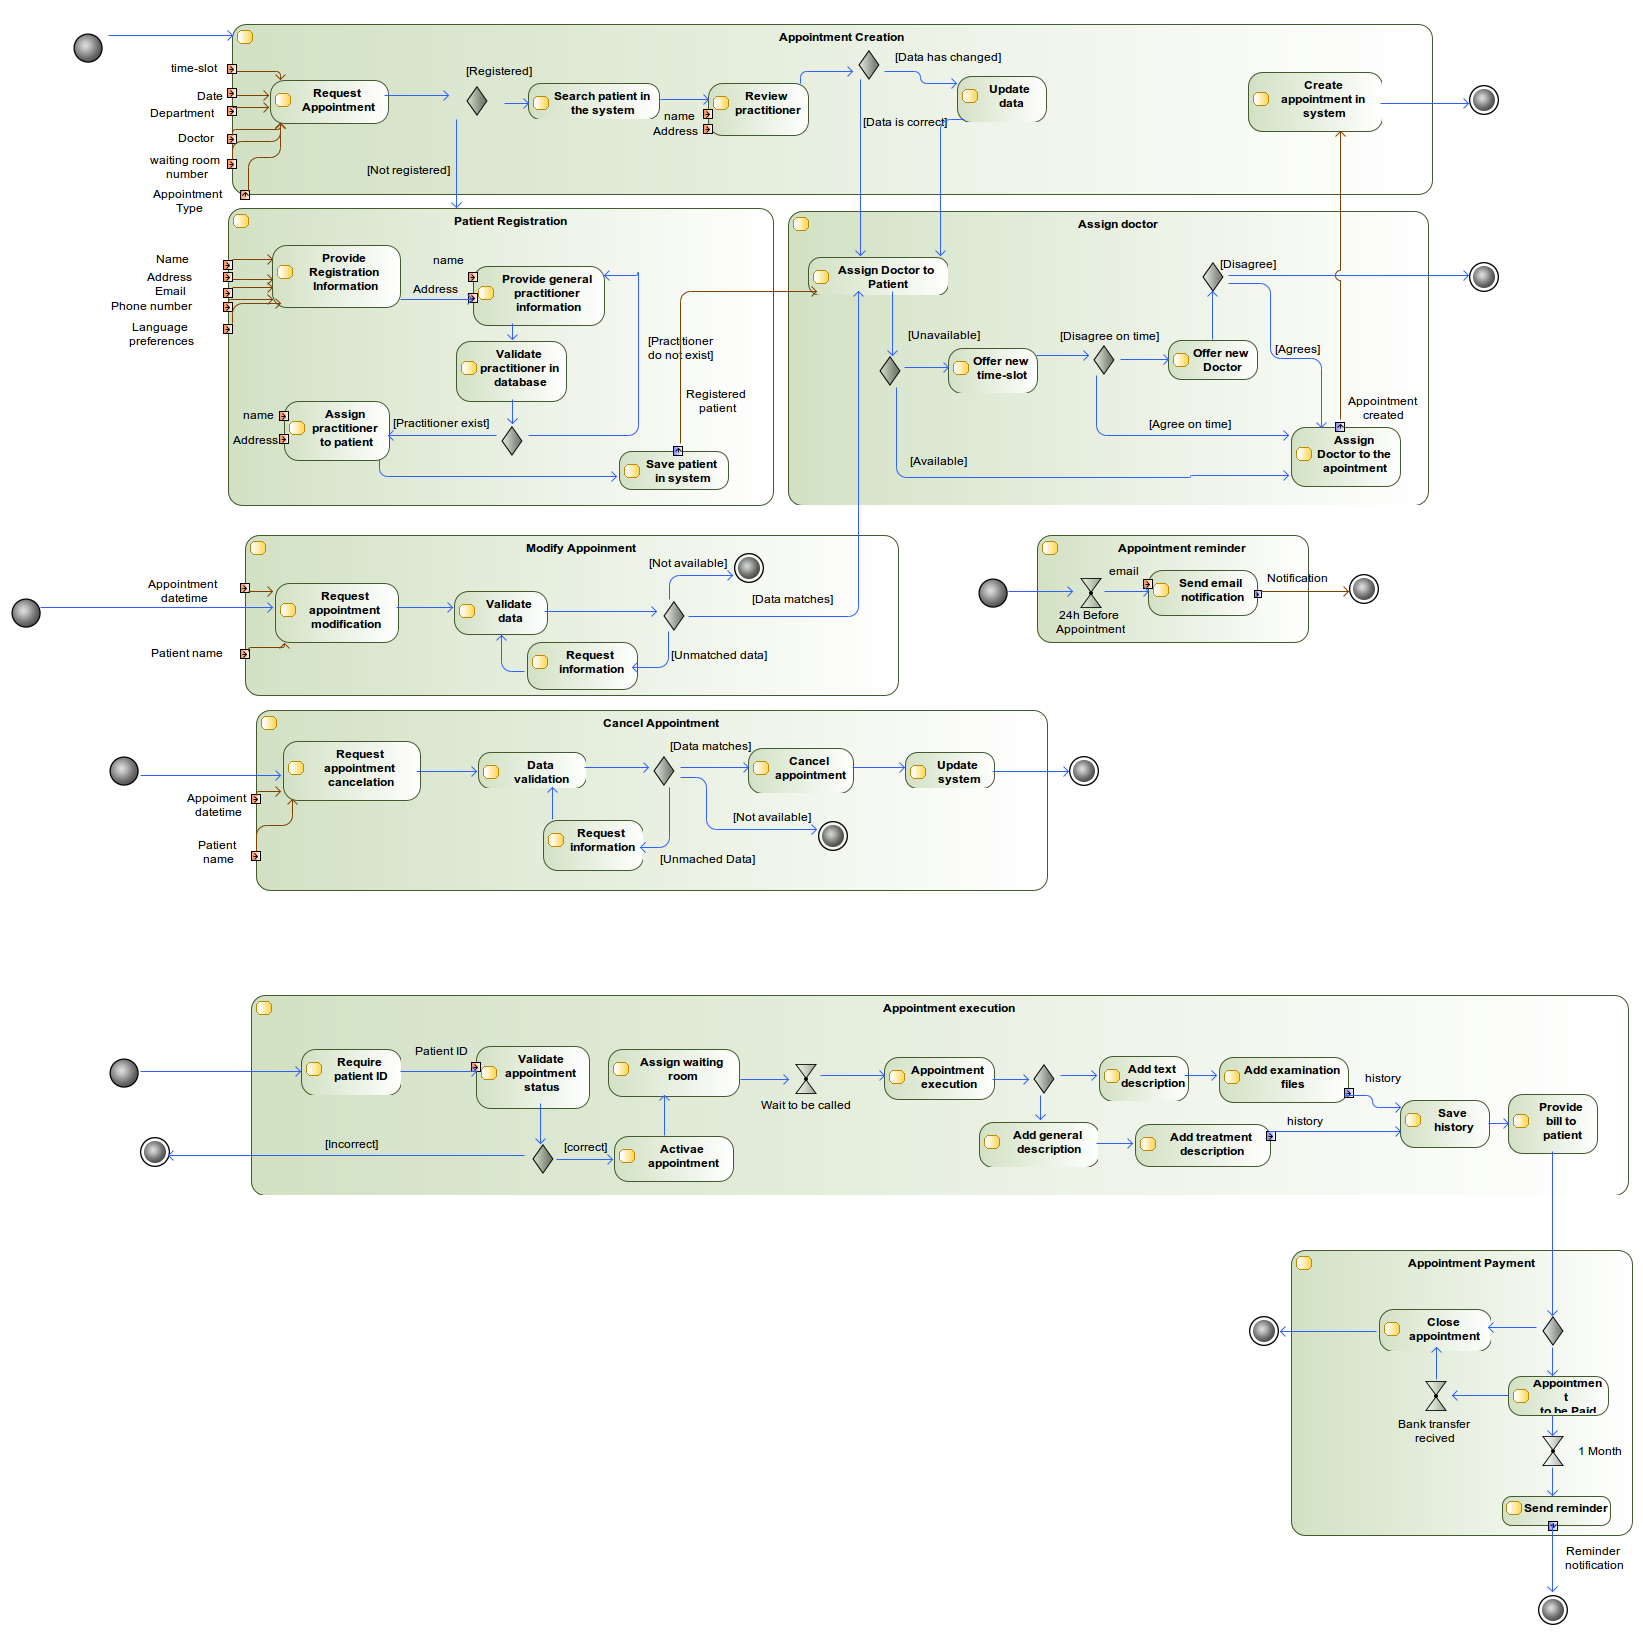
\includegraphics[width=1\linewidth]{./img/Activity.png}
                \setcaptioncitation{self-made}
                \caption{Distributed Computing Implementation.}
                \label{fig:architecture}
            \end{figure}
            \section{State Diagram}
            In this project, we tried to go further with the implementation by combining concepts that we learned in previous courses of the master, such as Web technologies and Databases.  
            We tried to simulate in a "real case" environment, where several devices with different applications or different back-end (e.g. mobile application in Python and web application in Nodejs) are used to collect a specific information and save it in a pre-defined database.
    
            \begin{figure}[H]
                \centering 
                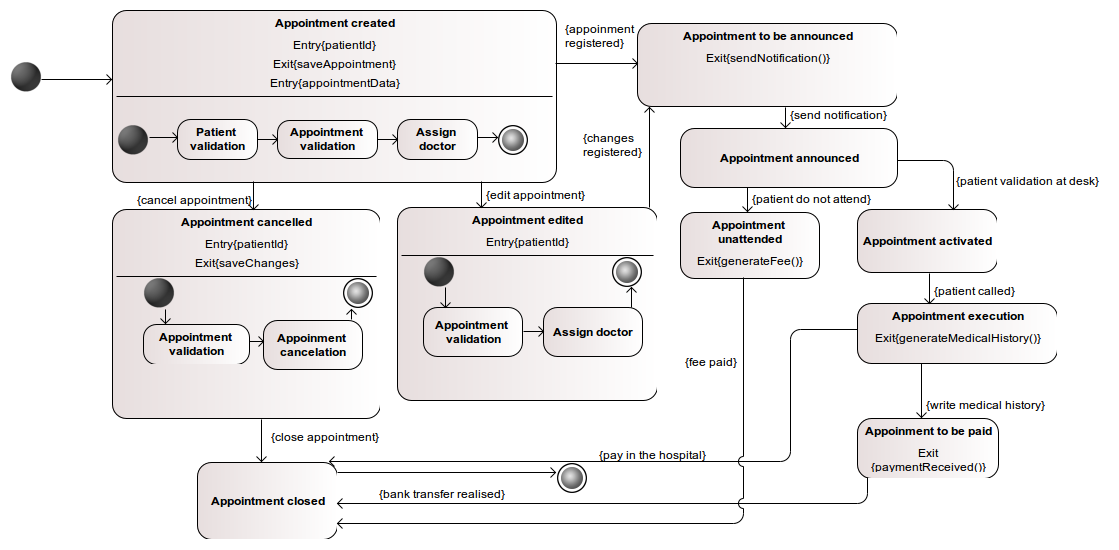
\includegraphics[width=1\linewidth]{./img/state.png}
                \setcaptioncitation{self-made}
                \caption{Distributed Computing Implementation.}
                \label{fig:architecture}
            \end{figure}
    
        
    \end{document}